
\documentclass[a4paper]{article} %
\usepackage{graphicx,amssymb} %

\usepackage{soul}

\textwidth=15cm \hoffset=-1.2cm %
\textheight=25cm \voffset=-2cm %

\newtheorem{prp}{Proposition}
\newtheorem{lmm}{Lemma}
\newtheorem{thr}{Theorem}
\newtheorem{dfn}{Definition}
\newtheorem{rmr}{Note}
\newtheorem{crl}{Corollary}
\newtheorem{ejemplo}{Example}
\newtheorem{notaci�n}{Notation}
\newtheorem{conjecture}{Conjecture}

\newcommand{\K}{\mathbb{K}}
\newcommand{\N}{\mathbb{N}}
\newcommand{\Z}{\mathbb{Z}}
\newcommand{\Q}{\mathbb{Q}}
\newcommand{\R}{\mathbb{R}}
\newcommand{\C}{\mathbb{C}}
\newcommand{\gothic}{\mathfrak}

\pagestyle{empty} %

\date{} %

\def\keywords#1{\begin{center}{\bf Keywords}\\{#1}\end{center}} %

\def\titulo#1{\title{#1}} %
\def\autores#1{\author{#1}} %

% Please, do not change any of the above lines








\begin{document}

% Type down your paper title
\titulo{Obtaining combinatorial structures associated with low-dimensional Leibniz algebras}

% Authors
\autores{Manuel Ceballos, Juan N\'u\~nez \\ %
       University of Seville (Spain) \\ \\ % Affiliation 1
       \'Angel F. Tenorio \\ % If any other author with different Affilation
       Pablo de Olavide University (Spain) \\ \\ % Affiliation 2 (if needed)
       % New author \\
       % New affiliation \\
       % Add authors and affiliation as needed
       \tt{mceballos@us.es} % Only one corresponding e-mail
       }%


\maketitle

\thispagestyle{empty}



% The abstract

\begin{abstract}
In this paper, we analyze the relation between Leibniz algebras and combinatorial structures. More concretely, we study the properties to be satisfied by (pseudo)digraphs so that they are associated with low-dimensional Leibniz algebras.
%We show some results and a related algorithmic method implemented with Maple $12$.
We present some results related to this association and show an algorithmic method to obtain them, which has been  implemented with Maple.

\end{abstract}

\keywords{%Digraph,
Pseudodigraph, Combinatorial structure, Leibniz algebra, Structure Theory, Algorithm
} % Write down at least 3 Keywords




\section{Introduction}\label{intro}

Leibniz algebras were introduced at the beginning of the 1990s by J.-L. Loday \cite{Loday}.
They are a particular case of non-associative algebras and provide a non-commutative generalization of Lie algebras.
There exists extensive research on these algebras due to their many applications in Engineering, Physics and Applied Mathematics. However, some aspects of Leibniz algebras remain unknown. In fact, the classification of nilpotent and solvable algebras is still an open problem.
%\hl{To achieve this purpose, mathematicians have dealt during the last decades with different links between solvable  algebras and other fields.}

Graph Theory is also very important and useful due to its many uses as a tool for other subjects. Our main goal is to extend the study and analysis of the relations between Graph Theory and Lie algebras proposed in \cite{CFN,CNT4}, but this time to the case of Leibniz algebras.

%In our opinion, the tools and results  dealt with  in this article are very useful and helpful to advance in understanding the relation between Leibniz algebras and simplicial complexes, since  the classification of combinatorial structures may involve an easier method to solve the  classification problem of Leibniz algebras  by means of the classification of their associated combinatorial structures.



\section{Preliminaries}\label{prel}

We  show some preliminary concepts  on Leibniz algebras, bearing in mind that the reader can consult \cite{Loday} as an introductory paper.

\begin{dfn}

A {\em Leibniz algebra} $\mathcal{L}$ over a field ${\K}$ is a vector space with a second inner bilinear composition law $[\cdot,\cdot]$, which verifies the so-called Leibniz identity
$$[[X,Y],Z]-[[X,Z],Y]-[X,[Y,Z]]=0, \,\, \forall \, X,Y,Z \in \mathcal{L}$$
>From now on, we will denote $L(X,Y,Z)=[[X,Y],Z]-[[X,Z],Y]-[X,[Y,Z]]$.

If, in addition, is verified that $[X,X]=0$, for all $X \in \mathcal{L}$, the Leibniz algebra is also a {\em Lie algebra}. In this case, it is satisfied that $[X,Y]=-[Y,X]$ and the Leibniz identity is equivalent to the Jacobi identity.

\end{dfn}

\begin{dfn}

Given a basis $\{e_i\}_{i=1}^n$ of an $n$-dimensional Leibniz algebra  $\mathcal L$, its {\em structure constants} are defined by $[e_i,e_j]=\sum_{h=1}^n c_{i,j}^h
e_h$, for  $1 \leq i, j \leq n$.


\end{dfn}

%\begin{dfn}
%
%A Lie algebra is semisimple if it is not abelian and does not
%contain any proper abelian ideal.
%
%\end{dfn}


\begin{dfn}
The {\em derived} and {\em central series} of a finite-dimensional Leibniz algebra $\mathcal{L}$ are
{\small$$\mathcal{L}_1= \mathcal{L}, \
\mathcal{L}_2=[\mathcal{L},\mathcal{L}], \ \dots,
\ \mathcal{L}_k=[\mathcal{L}_{k-1},
\mathcal{L}_{k-1}], \ \dots \quad {\rm and} \quad
\mathcal{L}^1= \mathcal{L}, \
\mathcal{L}^2=[\mathcal{L},\mathcal{L}], \ \dots,
\ \mathcal{L}^k=[\mathcal{L}^{k-1},
\mathcal{L}], \ \dots$$}
 So, $\mathcal{L}$ is
called $(m-1)$-step {\em solvable} (resp. {\em nilpotent}) if there exists $m\in\mathbb N$ such that
$\mathcal{L}_m = %\equiv
\{0\}$ and $\mathcal L_{m-1}\neq\{0\}$ (resp. $\mathcal{L}^m = %\equiv
\{0\}$ and $\mathcal L^{m-1}\neq\{0\}$).

\end{dfn}

%\begin{dfn}
%
%Given $n\in\mathbb{N}\setminus\{1\}$, Lie algebra $\mathfrak{h}_n$ (resp. $\mathfrak{g}_n$) is the solvable (resp. nilpotent) matrix algebra consisting of $n\times n$ upper-triangular matrices (resp. strictly upper-triangular matrices).
%
%\end{dfn}
%
%\begin{dfn}
%
%Given $k\in\mathbb{N}$, {\it Heisenberg algebra} $\mathfrak{H}_{k}$ is the $(2k+1)$-dimensional Lie algebra having the law $[e_{2i},e_{2i+1}]=e_1$ for $i=1,\dots,k$ with respect to a basis $\{e_i\}_{i=1}^{2k+1}$.
%
%\end{dfn}
%
%\begin{dfn}
%
%Given $k \in \mathbb{N}$ with $k \ge 3$, {\it model filiform Lie algebra}~$\mathfrak{f}_k$ is the $k$-dimensional Lie algebra such that its law, with respect to certain basis $\{e_i\}_{i=1}^{k}$, is $[e_1,e_h]=e_{h-1}$ for $3\le h \le k$.
%
%
%\end{dfn}



\section{Associating combinatorial structures with Leibniz algebras}
\label{Associating}

Let $\mathcal{L}$ be a $n$-dimensional Leibniz algebra with basis $\mathcal{B}=\{e_i\}_{i=1}^n$. Its structure constants correspond to $[e_i,e_j]=\sum_{h=1}^n c_{i,j}^h e_h$ and, hence, the pair $(\mathcal{L},\mathcal{B})$ is associated with a combinatorial structure by the following procedure

\begin{itemize}
\item [a)] For each $e_i \in \mathcal{B}$, we draw a vertex $i$.

\item [b)] For every vertex $i$ verifying $[e_i,e_i] \neq 0$, we draw a loop such that its weight is an $n$-tuple given by $(c_{i,i}^1,c_{i,i}^2, \ldots, c_{i,i}^n)$.

%\begin{figure}[htp]
%\begin{center}
%\includegraphics[width=4cm]{loop.eps}
%\caption{Loop over a vertex $i$.}\label{loop}
%\end{center}
%\end{figure}

\item [c)] Given two vertices $i$, $j$ verifying $(c_{i,j}^j,c_{j,i}^j) \neq (0,0)$, we draw a directed edge from vertex $i$ to $j$ whose weight is given by the pair  $(c_{i,j}^j,c_{j,i}^j)$.

%Given two vertices $i < j$ verifying $(c_{i,j}^j,c_{j,i}^j) \neq (0,0)$, we draw a directed edge from vertex $i$ to $j$ whose weight is given by the pair  $(c_{i,j}^j,c_{j,i}^j)$. If $(c_{i,j}^i,c_{j,i}^i) \neq (0,0)$, we draw another directed edge from $j$ to $i$ with weight $(c_{i,j}^i,c_{j,i}^i)$.

%\begin{figure}[htp]
%\begin{center}
%\includegraphics[width=3cm]{loop.eps}  \hspace{0.2cm}  \includegraphics[width=4cm]{directed_edge.eps}
%\caption{Loop over a vertex $i$ and a directed edge.}\label{directed_edge}
%\end{center}
%\end{figure}

%
%
%\begin{figure}[h!]
%%
%\begin{minipage}[t]{.20\linewidth}
%\noindent
%\centering\includegraphics[width=1.01\linewidth]{loop.eps}
%\caption{Loop over a vertex $i$.}\label{full_triangle}
%\end{minipage}
%%
%\hfill
%%
%\begin{minipage}[t]{.39\linewidth}
%\noindent
%\centering
%\includegraphics[width=.9\linewidth]{directed_edge.eps}
%\caption{Directed edge.}
%\label{sharing}
%\end{minipage}
%%
%\end{figure}

\item [d)] Given three vertices $i < j < k$ such that $(c_{i,j}^k, c_{j,i}^k, c_{j,k}^i, c_{k,j}^i, c_{i,k}^j, c_{k,i}^j)\neq (0,0,0,0,0,0)$, we draw a full triangle $ijk$ such that the edges $ij$, $jk$ and $ik$ have weights $(c_{i,j}^k,c_{j,i}^k)$, $(c_{j,k}^i,c_{k,j}^i)$ and $(c_{i,k}^j,c_{k,i}^j)$, respectively. Moreover,

\begin{itemize}

\item [d1)] we use a discontinuous line (named {\em ghost edge}) for edges with weight $(0,0)$.

\item [d2)] If two triangles $ijk$ and $ijl$ satisfy $(c_{i,j}^k,c_{j,i}^k) = (c_{i,j}^l,c_{j,i}^l)$, draw only one edge between vertices $i$ and $j$ shared  by  both triangles.

\end{itemize}

%\begin{figure}[htp]
%\begin{center}
%\includegraphics[width=5cm]{full_triangle.eps}  \hspace{0.2cm}  \includegraphics[width=6cm]{shared_edge.eps}
%\caption{Full triangle and two triangles sharing an edge.}\label{directed_edge}
%\end{center}
%\end{figure}

\begin{figure}[htp]
\begin{center}
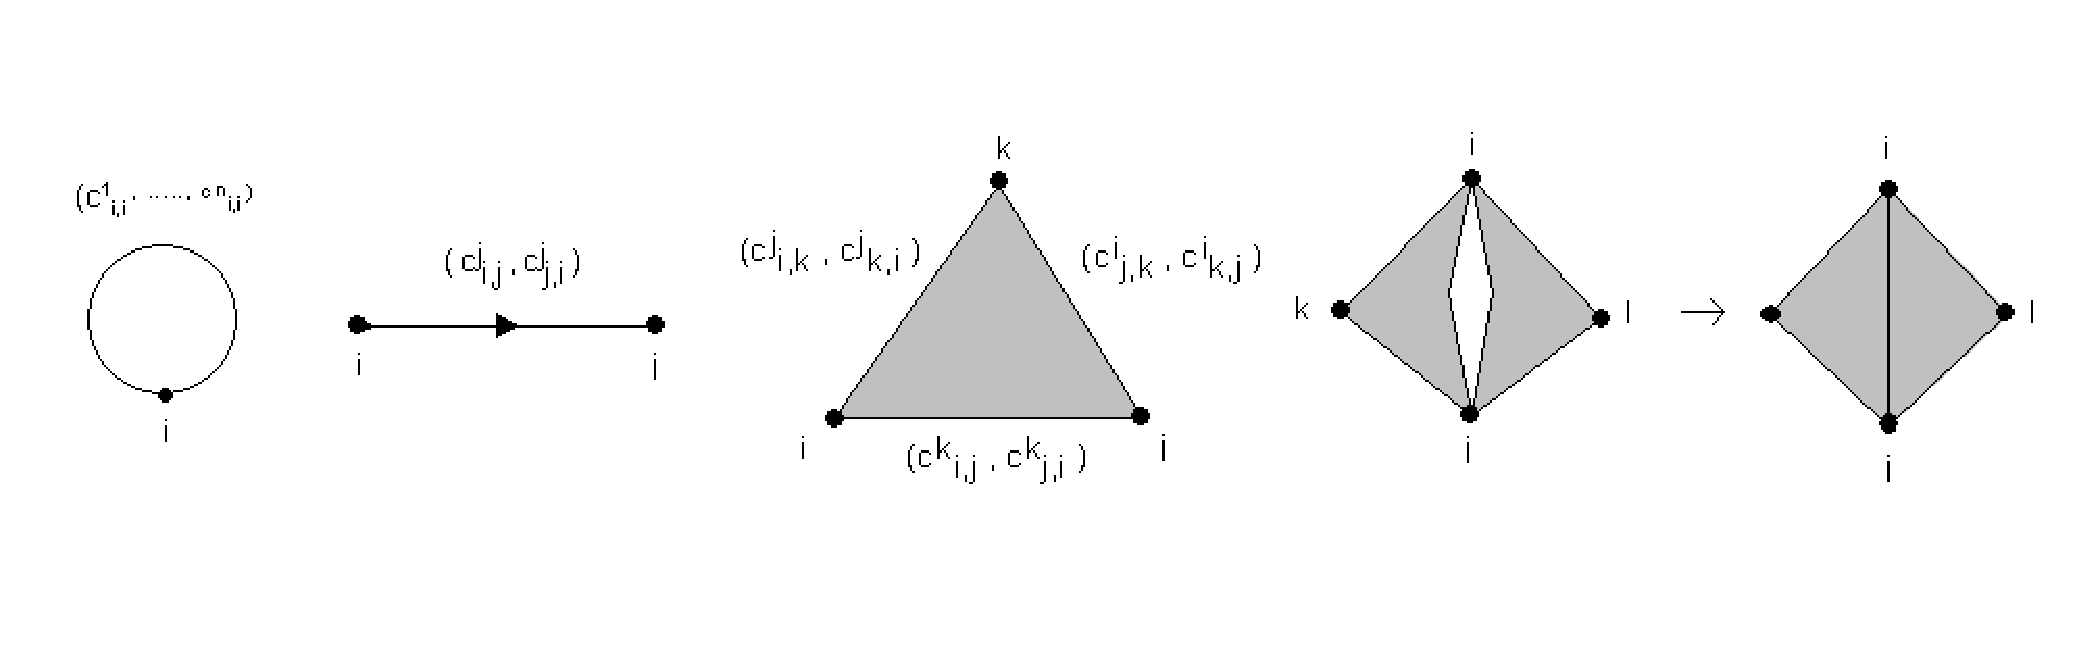
\includegraphics[width=12cm]{grupo-1.eps}

\vspace{-0.7cm}

\caption{Loop, directed edge, full triangle and two triangles sharing an edge.}\label{directed_edge}
\end{center}
\end{figure}


%
%
%\begin{figure}[h!]
%%
%\begin{minipage}[t]{.40\linewidth}
%\noindent
%\centering\includegraphics[width=1.01\linewidth]{full_triangle.eps}
%\caption{Full triangle.}\label{full_triangle}
%\end{minipage}
%%
%\hfill
%%
%\begin{minipage}[t]{.69\linewidth}
%\noindent
%\centering
%\includegraphics[width=.9\linewidth]{shared_edge.eps}
%\caption{Two triangles sharing an edge.}
%\label{sharing}
%\end{minipage}
%%
%\end{figure}



\end{itemize}

\section{Leibniz algebras and (pseudo)digraphs}

In this section, we study the structure of digraphs associated with low-dimensional Leibniz algebras. For each case, we will study the type of Leibniz algebra according to the solvability of this algebra. To be associated with a (pseudo)digraph $G$, a given Leibniz algebra $\mathcal{L}$ with basis $\mathcal B=\{e_i\}_{i=1}^n$ has the following law
\begin{equation}\label{bracketsleibniz} [e_i,e_j]=c_{i,j}^i e_i + c_{i,j}^j e_j, \,\, 1 \leq i \neq j \leq n; \quad [e_k,e_k]=\sum_{h=1}^n c_{k,k}^h e_h \end{equation}
\noindent since these brackets avoid the appearance of full triangles in  $G$.



\begin{prp}\label{notLienotLeibniz}

Every digraph %containing one of the configurations
admitting some configuration of \cite[Fig. 9]{CFN} as a subdigraph is not associated with any Leibniz algebra.

\end{prp}


%Now, we show several results depending on the dimension of the Leibniz algebra. For each case, we study the type of graphs associated.

\begin{prp}

The abelian Leibinz algebra is the only one of dimension 1, associated with a digraph.
%The unique $1$-dimensional Leibniz algebra associated with a graph is the abelian one.

\end{prp}

\begin{prp}

Let $\mathcal{L}$ be a $2$-dimensional Leibniz algebra associated with a connected pseudodigraph $G$. Then,
the configuration $d)$ shown in Figure \ref{config_dim2} is forbidden in $G$. In fact, $G$ must present one of the remaining configurations in that figure. Moreover, it is verified that


%
%Then, $G$ must present one of the configurations in Figure \ref{config_dim2}, up to permutation of labels
%
%
%
%, being forbidden any other configuration. Moreover, it holds that

%the configuration $d)$ %shown
%in Figure \ref{config_dim2} is forbidden in $G$. In fact, $G$ must present one of the remaining configurations in %that figure
%Figure \ref{config_dim2}, up to permutation of labels. Moreover, it holds %is verified
%that


\begin{figure}[htp]
\begin{center}
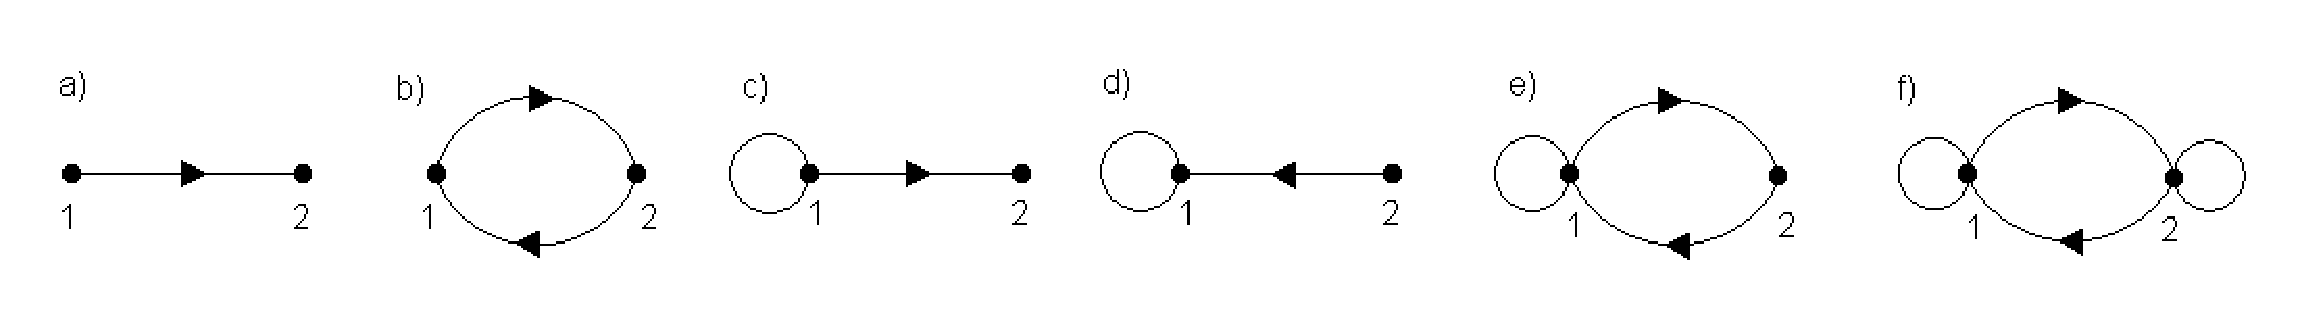
\includegraphics[width=14cm]{config_dimen2.eps}
\vspace{-1.5em}
\caption{Pseudodigraphs with two vertices and associated with Leibniz algebras.} \label{config_dim2}
\end{center}
\end{figure}




\begin{itemize}

\item Configurations a) and c) are associated with $2$-step solvable non-nilpotent Leibniz algebras.

\item Configuration b) is always associated with 2-step solvable non-nilpotent Lie algebras (i.e. only commutative Leibniz algebras).

\item Configurations e) and  f) are associated with a $2$-step nilpotent Leibniz algebras.

\end{itemize}


\end{prp}

%Next, we show several examples with Configuration f).


\begin{ejemplo}
Let $\mathcal{L}$ be the Leibniz algebra with brackets $[e_2,e_1]=e_2$ associated with Configuration a). In this case, $\mathcal{L}_2 =\mathcal{L}^2 =\langle e_2 \rangle$, whereas $\mathcal{L}^i=\mathcal{L}_2$ and $\mathcal{L}_i=0$ , for all $i \geq 3$. Therefore, $\mathcal{L}$ is 2-step solvable, non-nilpotent.

\end{ejemplo}

\begin{ejemplo}
We consider the Leibniz algebra $\mathcal{L}$ with law $[e_1,e_1]= -e_1 -e_2$, $[e_1,e_2]= e_1+e_2$ associated with Configuration e). In this case, $\mathcal{L}^2 =\mathcal{L}_2=\langle e_1+e_2\rangle$ and $\mathcal L_3=\mathcal L^3=0$. Hence, $\mathcal{L}$ is 2-step nilpotent.

\end{ejemplo}

\begin{ejemplo}

Let $\mathcal{L}$ be the Leibniz algebra with brackets $[e_1,e_1]=[e_2,e_2]=-e_1-e_2, [e_1,e_2]=[e_2,e_1]=e_1+e_2$, associated with Configuration f). For this algebra, $\mathcal{L}_2 =\langle e_1+e_2 \rangle$, $\mathcal{L}_3=\mathcal{L}^3=\{0\}$. So, $\mathcal{L}$ is $2$-step nilpotent.

\end{ejemplo}


\begin{prp}\label{Leibnizdim3}

%Let $\mathcal{L}$ be a $3$-dimensional Leibniz algebra associated with a pseudodigraph $G$.
%Then, $G$ corresponds to %must present
%one of the configurations in Figure \ref{config_dim3_pseudo}, up to permutation of labels.
Let $\mathcal{L}$ be a $3$-dimensional Leibniz algebra associated with a connected pseudograph $G$ including some loop.
Then, $G$ must present one of the configurations in Figure \ref{config_dim3_pseudo} up to permutation of labels. Any other pseudodigraph is forbidden in $G$.

\begin{figure}[htp]
\begin{center}
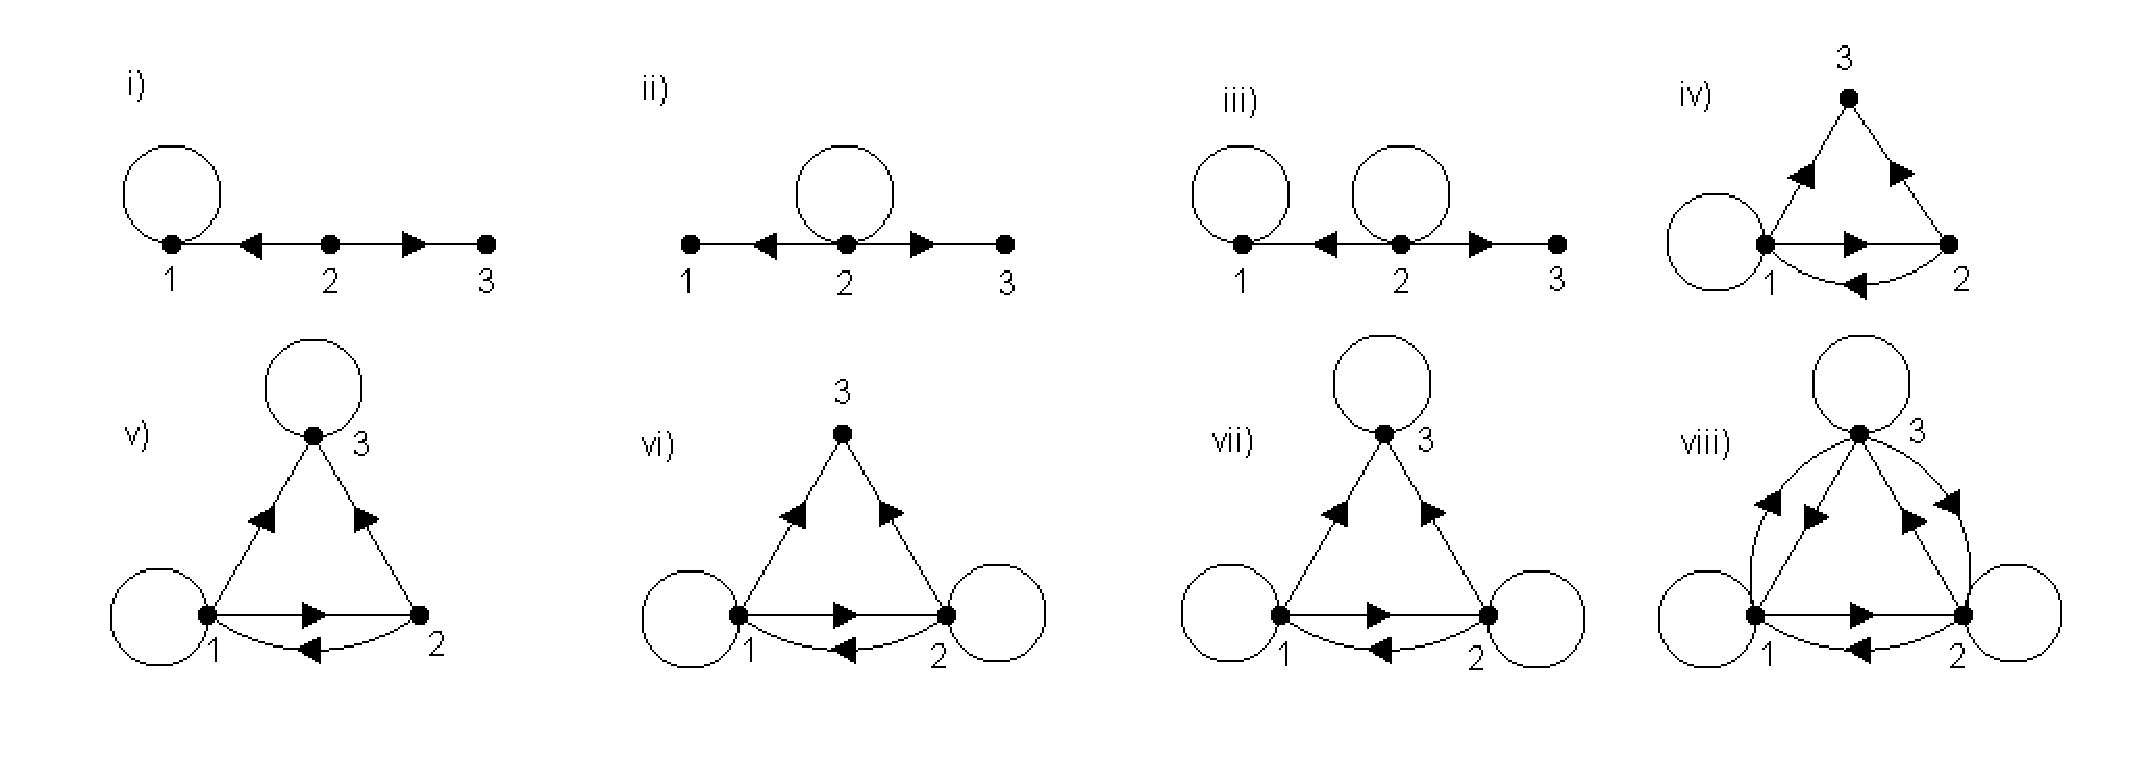
\includegraphics[width=11cm]{config_dim3_pseudo.eps}
\vspace{-1.5em}
\caption{Pseudodigraphs with three vertices, associated with Leibniz algebras, not being Lie algebras.} \label{config_dim3_pseudo}
\end{center}
\end{figure}


%\begin{figure}[htp]
%\begin{center}
%\includegraphics[width=14cm]{config_dim3_pseudo_prohibidas-.eps}
%\vspace{-1.5em}
%\caption{Forbidden pseudo\hl{di}graphs with three vertices.} \label{config_dim3_pseudo_prohibidas}
%\end{center}
%\end{figure}


\end{prp}

%\vspace{-0.7cm}


\begin{prp}

Let $G$ be a pseudodigraph formed by the first configuration of \cite[Fig. 15]{CFN} with loops. Then $G$ is associated with a solvable non-nilpotent Leibniz algebra.

\end{prp}

\begin{prp}

Let $G$ be a pseudodigraph formed by the second configuration of \cite[Fig. 15]{CFN} with loops. Then, $G$ is associated with a Leibniz algebra if and only if $G$ has a loop on each vertex incident with a double edge.

\end{prp}

\section{Implementation and complexity% of a method
 for the Leibniz identity}

Now, we show the algorithmic method that we have used in the previous section to evaluate the Leibniz identity in order to find out the allowed and forbidden configurations and the restrictions over the weights of the edges. Regarding this, we have implemented our algorithm using the symbolic computation package MAPLE%~$12$.
, working the implementation in version 12 or higher%\hl{Although we have used this version, we would like to point out that it is possible to run the method by using any other version, like MAPLE~$17$, which is the last one
. To do this, we 
will use the libraries {\tt linalg},  {\tt combinat}, {\tt GraphTheory} and {\tt Maplets[Elements]} to activate commands related to Linear and Combinatorial Algebra, Graph Theory and the last one to display a message so that the user introduces the required input in the first subprocedure. So, we start considering a vector space $\mathcal{L}$ with basis $\mathcal{B}$ and the type of brackets expressed in (\ref{bracketsleibniz}) and give the following steps:

\begin{enumerate}
\item Computing the bracket product between two arbitrary basis vectors in $\mathcal B$.


This first subprocedure is called {\tt law} and computes the bracket between two arbitrary basis vectors in $\mathcal B$. It
 receives the subindexes of two basis vectors in $\mathcal B$. A conditional sentence is introduced to determine each non-zero bracket. The user has to complete the implementation depending on the law of $\mathcal{L}$, so we have added a sentence at the beginning of the implementation, reminding of this fact. Before running any other sentence, we restart all the variables by using the command {\tt restart}. Moreover, we save the value of variable {\tt dim} (the dimension) with the command {\tt assign}.

{\footnotesize
\begin{verbatim}
> maplet:=Maplet(AlertDialog("Don't forget to introduce non-zero brackets and the dimension in
subprocedure law",'onapprove'=Shutdown("Continue"),'oncancel'=Shutdown("Aborted"))):
> Maplets[Display](maplet):
> assign(dim,...):
> law:=proc(i,j)
>   if (i,j)=... then ...;
>   elif ....
>   else 0; end if;
> end proc;
\end{verbatim}}



\item Evaluating the bracket between two vectors expressed as a linear combination of vectors from basis $\mathcal B$.

We implement the subprocedure called {\tt bracket} to compute the product between two arbitrary vectors of $\mathcal{L}$, which are expressed as linear combinations of the vectors in $\mathcal{B}$. The subprocedure {\tt law} is called in the implementation.
{\footnotesize
\begin{verbatim}
> bracket:=proc(u,v,n)
>   local exp; exp:=0;
>   for i from 1 to n do
>      for j from 1 to n do
>         exp:=exp + coeff(u,e[i])*coeff(v,e[j])*law(i,j);
>      end do;
>   end do;
>   exp;
> end proc:
\end{verbatim}}


\item Imposing the Leibniz identity and solving the corresponding system of equations.

Next, we show the implementation of the main procedure called {\tt Leibniz}, which checks if the vector space ${\mathcal L}$ is or not a Leibniz algebra. This procedure receives as input the dimension $n$ of the vector space $\mathcal{L}$ and returns the solution of a system of equations obtained from imposing the Leibniz identity in $\mathcal{L}$. If the system has no solution, then we can conclude that the vector space $\mathcal{L}$ is not a Leibniz algebra. Otherwise, we will obtain the conditions over the structure constants $c_{i,j}^k$ so that $\mathcal{L}$ is a Leibniz algebra.
 %For the implementation we use the previous subroutine and define four local variables: first, the lists {\tt L} and {\tt M}, which are used to save all the possible permutations of the first $n$ numbers taken three by three; the variable {\tt N}, which is defined in order to save all the expressions from the Leibniz identity; and, finally, the list {\tt P} that solves the resulting system of equations.

%{\footnotesize
%\begin{verbatim}
%> Leibniz:=proc(n)
%> local L,M,N,P; L:=[];M:=[];N:=[];P:=[];
%> for i from 1 to n do L:=[op(L),i,i,i]; end do;
%> M:=permute(L,3); for j from 1 to nops(M) do
%> eq[j]:=bracket(bracket(e[M[j][1]],e[M[j][2]],n),e[M[j][3]],n)-
%>        bracket(bracket(e[M[j][1]],e[M[j][3]],n),e[M[j][2]],n)-
%>        bracket(e[M[j][1]],bracket(e[M[j][2]],e[M[j][3]],n),n);
%> end do; N:=[seq(eq[k], k=1..nops(M))]; for k from 1 to nops(N) do
%> for h from 1 to n do P:=[op(P),coeff(N[k],e[h])=0]; end do; end do;
%> return solve(P); end proc:
%\end{verbatim}}

{\footnotesize
\begin{verbatim}
> Leibniz:=proc(n)
>   local L,M,N,P;
>   L:=[];M:=[];N:=[];P:=[];
>   for i from 1 to n do
>     L:=[op(L),i,i,i];
>   end do;
>   M:=permute(L,3);
>   for j from 1 to nops(M) do
>     eq[j]:=bracket(bracket(e[M[j][1]],e[M[j][2]],n),e[M[j][3]],n)-
>            bracket(bracket(e[M[j][1]],e[M[j][3]],n),e[M[j][2]],n)-
>            bracket(e[M[j][1]],bracket(e[M[j][2]],e[M[j][3]],n),n);
>   end do;
>   N:=[seq(eq[k], k=1..nops(M))];
>   for k from 1 to nops(N) do
>      for h from 1 to n do
>        P:=[op(P),coeff(N[k],e[h])=0];
>      end do;
>   end do;
>   solve(P);
> end proc:
\end{verbatim}}

%\item Representing digraphs associated with Leibniz algebras.
%
%In this step, we represent the digraph associated with the Lie algebras obtained in the previous step. In order to do so, we must define two sets: the vertex set $V$, containing all the natural numbers up to $n$; and the edge set, $E$. In this last set, and according to the brackets defined in (\ref{bracketslie}), we must introduce the weight of the edges.
%
%{\footnotesize
%\begin{verbatim}
%> V:=[seq(i,i=1..dim)];
%> E:={[[i,j],c_{i,j}^j],[[j,i],c_{i,j}^i],...};
%\end{verbatim}}
%
%Finally, with the following orders we can represent the digraph
%
%{\footnotesize
%\begin{verbatim}
%> G:=Digraph(V,E): DrawGraph(G);
%\end{verbatim}}
%


\end{enumerate}


\begin{ejemplo}\label{ejemplo1}

Now, we show an example with the configuration i) from Figure \ref{config_dim3_pseudo}. We consider the $3$-dimensional vector space $\mathcal{L}$ with brackets
$$[e_1,e_1]=\sum_{i=1}^3 c_{1,1}^i e_i; \, \, [e_j,e_2]=c_{j,2}^j e_j, \, [e_2,e_j]=c_{2,j}^j e_j, \,{\rm for} \, j=1,3$$
First, we have to complete the implementation of the subprocedure {\tt law} as follows


{\footnotesize\begin{verbatim}
> maplet:=Maplet(AlertDialog("Don't forget to introduce non-zero brackets and the dimension in
subprocedure law",'onapprove'=Shutdown("Continue"),'oncancel'=Shutdown("Aborted"))):
> Maplets[Display](maplet):
> assign(dim,3):
> law:=proc(i,j)
>   if (i,j)=(1,1) then c111*e[1]+c112*e[2]+c113*e[3];
>   elif (i,j)=(1,2) then c121*e[1];
>   elif (i,j)=(2,1) then c211*e[1];
>   elif (i,j)=(2,3) then c233*e[3];
>   elif (i,j)=(3,2) then c323*e[3];
>     else 0;
>   end if;
> end proc:
\end{verbatim}}

After that, we must run the subprocedure {\tt bracket} and the procedure {\tt Leibniz}. Now, we evaluate this main procedure over the variable {\tt dim}

{\footnotesize\begin{verbatim}
> Leibniz(dim);
>      {c111=0,c112=0,c113=c113,c121=-c211,c211=c211,c233=0,c323=-2*c211}
\end{verbatim}}

So, we obtain those restrictions for the weights of the edges in configuration i) from Figure \ref{config_dim3_pseudo}.

\end{ejemplo}


Next, we compute the complexity of the algorithm. To do so, we consider the number of
operations carried out in the worst case. We use the big $O$ notation to express
the complexity. To recall the big $O$ notation, the reader can consult \cite{Wil86}: given two functions
$f,g:\mathbb{R}\to\mathbb{R}$, we could say that $f(x)=O(g(x))$ if and
only if there exist $M\in\mathbb R^+$ and $x_0\in\mathbb R$ such that  $|f(x)|<M\cdot |g(x)|$,
for all $x>x_0$.

We denote by $N_i(n)$ the number of operations when considering the step $i$. This function depends on the dimension $n$ of the Lie algebra.
Table~\ref{comp} shows the number of computations and the complexity of each step, as well as indicating the name of the procedure corresponding to each step.

\begin{table}[htp] \caption{Complexity and number of operations.}\label{comp}
\begin{center}
\begin{tabular}{|c|c|c|c|}
\hline Step & Procedure & Complexity & Operations \\
\hline 1 & {\tt law} & $O(n^2)$ & $N_1(n)=O\left(\frac{n(n-1)}{2}\right)$ \\
\hline 2 & {\tt bracket} & $O(n^4)$ & $N_2(n)=\displaystyle\sum_{i=1}^{n}\displaystyle\sum_{j=1}^{n} N_1(n)$ \\
\hline 3 & {\tt Leibniz} & $O(n^7)$       & $N_3(n)= O(n)+O(n^3)+ \displaystyle\sum_{i=1}^{n^3} N_2(n) + \displaystyle\sum_{j=1}^{n^3} \displaystyle\sum_{k=1}^{n} 1$ \\
\hline
\end{tabular}
\end{center}
\end{table}












\begin{thebibliography}{}

%\bibitem{Barnes} D. W. Barnes, On Levi's theorem for Leibniz algebras, Bull. Aust. Math. 86:2 (2012), 184--185.

\bibitem{CFN} A. Carriazo, L.M. Fern\'andez, J. N\'u\~nez, Combinatorial structures associated with Lie algebras of finite dimension, Linear Algebra Appl. 389 (2004), 43--61.

%\bibitem{CNT} M. Ceballos, J. N\'u\~nez, A.F. Tenorio, Complete triangular structures and Lie algebras, Int. J. Computer Math. 88:9 (2011), 1839--1851.
%
%\bibitem{CNT2} M. Ceballos, J. N\'u\~nez, A.F. Tenorio, Study of Lie algebras by using combinatorial structures, Linear Algebra Appl.  436 (2012), 349--363.
%
%\bibitem{CNT3}  M. Ceballos, J. N\'u\~nez, A.F. Tenorio, Combinatorial structures and lie algebras of upper-triangular matrices, Appl. Math. Lett.  25 (2012), 514--519.


\bibitem{CNT4} J. C\'aceres, M. Ceballos, J. N\'u\~nez, M.L. Puertas, A.F. Tenorio, Combinatorial structures of three vertices and Lie algebras, Int. J. Computer Math. 89:13--14 (2012), 1879--1900.

%\bibitem{Diestel}  R. Diestel, Graph Theory, 4th. Edition, Springer-Verlag, Heidelberg, 2010.

%\bibitem{F-M} L.M. Fern\'andez, L. Mart\'in-Mart\'inez, Lie algebras associated with triangular configurations. Linear Algebra Appl. 407 (2005), 43--63.

%\bibitem{G-T} L. Yu Galitski and D.A. Timahsev, On classification of metabelian Lie algebras, J. Lie Theory 9 (1999), 125--156.

%\bibitem{Lev1905} E.E. Levi,  Sulla struttura dei gruppi finiti e continui, Atti. Accad. Sci. Torino 40 (1905), 551--565.

\bibitem{Loday} J.L. Loday, Une version non commutative des alg\`ebres de Lie: les alg\`ebres de Leibniz, Enseign. Math. (2), 39
(1993), pp. 269--293.

%\bibitem{MA} A.I. Malcev, Solvable Lie algebras. Trans. Amer. Math. Soc. Transl. 9 (1962), 228--262.

%\bibitem{Pr}  M. Primc, Basic representations for classical affine Lie algebras,  J. of Algebra 228 (2000), 1--50.

%\bibitem{Se} J.P. Serre, Alg\`ebres de Lie Semi-Simples Complexes, Benjamin Inc., New York, 1996.


%\bibitem{Var98} V.S. Varadarajan, Lie Groups, Lie Algebras and Their Representations, Springer, New York, 1984.

\bibitem{Wil86}  H.S.~Wilf, Algorithms and Complexity, Prentice Hall, Englewood Cliffs, 1986.

\end{thebibliography}



\end{document}





